\section{The Wanderer's Minuet}

The Wanderer's Minuet is conceptually similar to Mage's Ballad in that Repertoire procs will generate stacks to be used on the ability Pitch Perfect. However, Pitch Perfect can gain up to 3 charges, where each charge further increases potency. The Wanderer's Minuet is normally used during burst windows, so it must be accounted for whether or not Pitch Perfect (PP) was used inside the burst window or outside the burst window.\footnote{Medication lasts beyond the standard burst window. For simplicity of analysis and computation, any medication effects are ignored and will lead to a small negative bias in computed damage distributions.}  Any PP stacks not used in the burst window will carry over to the non-burst window, and must be accounted for.

To simplify analysis, the following assumptions are made:

\begin{itemize}
    \item PP with 3 stacks, PP3, is only ever used.
    \item The burst window will also include the first couple of GCDs which occur before party buffs go out as PP stacks can accumulate. Assuming the burst window happens on the 2nd GCD, it will be impossible to attain PP3 before the burst window actually begins.
    \item  The burst window will contain 2 Empyreal Arrows, guaranteeing 2 PP stacks. The non-burst window will contain 1 Empyreal Arrow, guaranteeing 1 PP stack. 
    \item Collisions, a scenario where 2 PP stacks are present and where a potential Repertoire proc and Empyreal Arrow usage are close enough that it would lead to overcapping, do not happen. 
\end{itemize}

The goal of the section is to derive a joint probability distribution for the number of PP3 procs in the burst window ($k^b_{pp3}$) and non-burst window ($k_{pp3}^{nb}$). Damage distributions for all valid PP3 proc pairs will be computed and their respective probabilities are weights when constructing a mixture distribution from eqn. \ref{eqn:dmg-mixture}.

The number of Repertoire procs, $k_r$, can be related to the number of PP3 procs in the burst window, $k^b_{pp3}$ by

\begin{equation}
    k^b_{pp3} = \left\lfloor \frac{k^b_r + n_{ea}^b }{3} \right\rfloor \label{eqn:wm-rep-to-pp-burst}
\end{equation}

where $n^b_{ea}$ is the number of Empyreal Arrow usages for the burst window. Since it is assumed only PP3 is used, the number of leftover PP procs in the burst window carried over to the non-burst window, $\ell$, can be expressed as

\begin{equation}
    \ell = k^b_r + n_{ea}^b \bmod 3
    \label{eqn:wm-proc-carryover}
\end{equation}

The joint probability distribution for $k_{pp3}$ PP3 procs in burst and a PP leftover count of $\ell$, sums over all Repertoire proc probabilities, but is constrained by eqn. \ref{eqn:wm-rep-to-pp-burst} ($n_{ea}^b = 2$) and eqn. \ref{eqn:wm-proc-carryover}.

\begin{equation}
    P^b_{pp3}(k^b_{pp3}, \ell; n^b_r, p_r) = 
    \sum_{\substack{i = 0 \\ \lfloor (i + 2) / 3 \rfloor = k_{pp3} \\ i + 2 \bmod 3 = \ell}}^{n_r^b}
    P_r(i; n_r^b, p_r)
\end{equation}

This summation aggregates probabilities of all Repertoire proc counts that yield exactly $k^b_{pp3}$ PP3 casts while leaving $\ell$ leftover stacks.

The distribution of non-burst PP3 procs must also account for all possible leftover PP values from the burst window in addition to all possible Repertoire procs in the non-burst window. The number of non-burst PP3 procs, including $\ell$ leftover procs from the burst window is

\begin{equation}
    k^{nb}_{pp3} = \left\lfloor \frac{k^{nb}_r + n_{ea}^{nb} + \ell}{3} \right\rfloor 
    \label{eqn:wm-rep-to-pp-nonburst}
\end{equation}

The non-burst window PP3 proc distribution for $n_{ea} = 1$ and $\ell$ PP stacks leftover from the burst window follows a similar sum constrained by eqn. \ref{eqn:wm-rep-to-pp-nonburst} with $n_{ea}^{nb} = 1$

\begin{equation}
\begin{split}
P^{nb}_{pp3}(k_{pp3}^{nb}, \ell; &n_{r}^{nb}, p_r) = \\
&\sum_{\substack{j = 0 \\ \lfloor (j + \ell + 1)/3\rfloor = k_{pp3}^{nb}}}^{n_r^{nb}}
P_r(j;n^{nb}_r, p_r)
\end{split}
\end{equation}

which filters and aggregates probabilities that result in $k^{nb}_{pp3}$ PP3 procs.

As both marginal distributions are independent random variables, the joint burst PP3 and non-burst PP3 is simply multiplicative and marginalizes out all possible burst leftover values

\begin{equation}
    \begin{split}
    P_{pp3}&(k^b_{pp3}, k^{nb}_{pp3}; n_r^b, n_r^{nb}, p_r) = \\
    & \sum_{\ell = 0}^{2} P^b_{pp3}(k^b_{pp3}, \ell; n^b_r, p_r) P^{nb}_{pp3}(k_{pp3}^{nb}, \ell; n_{r}^{nb}, p_r)
    \end{split}
\end{equation}

One implicit simplification is that the number of leftover PP procs from the \textit{non-burst} window is not calculated. While this could certainly be calculated, it also creates a 3D joint probability distribution and would considerably increase the number of unique proc tuples to iterate over.\footnote{Each new set of buffs increases the dimensionality of the joint probability distribution. For example, accounting for medication-only window would require enumerating over a 4D joint probability distribution.} Instead, a non-burst leftover PP stack of 1 is assumed. For $(k^b_{pp3} = 3, k^{nb}_{pp3} = 3)$, the non-burst leftover PP stack is set to 0, as no more PP stacks are achievable. The 2D joint PP3 proc distribution for $n_r^b = 8$ and $n_r^{nb} = 7$ is shown in Figure \ref{fig:wm-joint-pp3}.

\begin{figure}[H]
    \centering
    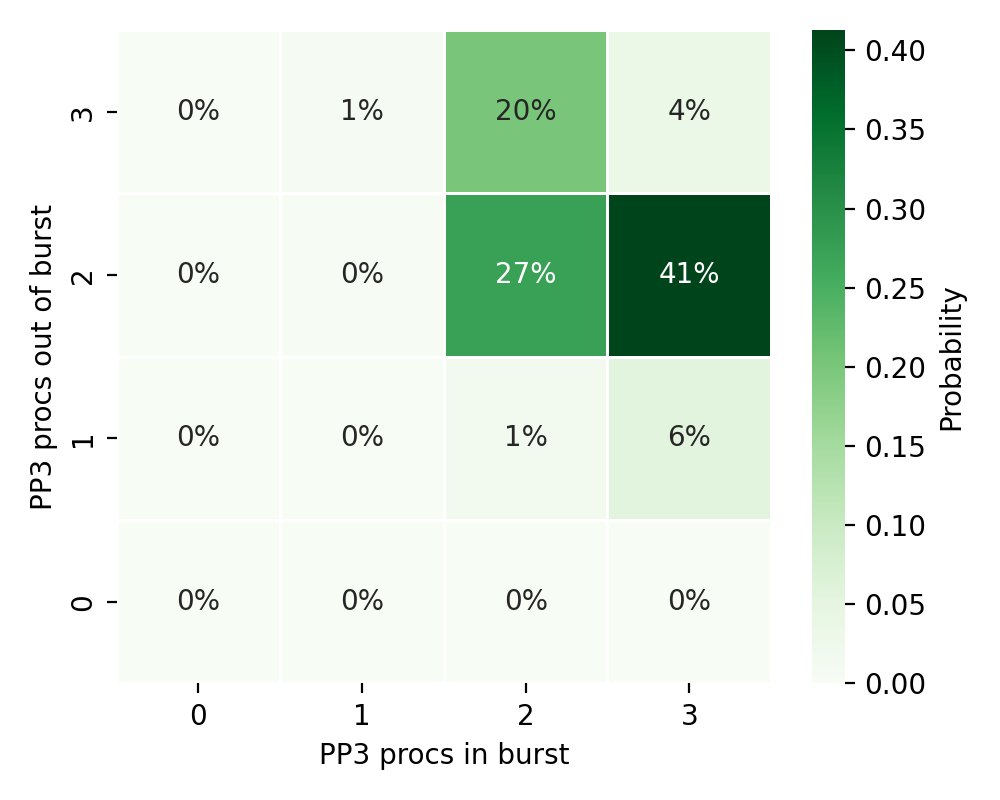
\includegraphics[scale=0.65]{img/wm-joint.png}
    \caption{Joint PP3 proc probability distribution during the burst window and outside of the burst window.}
    \label{fig:wm-joint-pp3}
\end{figure}

Pairs of 2 and 3 PP3 procs in each window are the most common, which makes sense as each tick of Repertoire has an 80\% chance of granting a PP stack. Getting more stacks during the burst window is slightly more likely, due to $n_{ea} = 2$. Getting 3 PP3 procs in each window is unlikely, as that would require every single Repertoire tick to grant a PP stack. The overall damage distribution accounting for PP3 procs is now a double sum to account for both PP3 proc windows:

\begin{equation}
\begin{split}
    P(D_{pp3}) = \sum_{i=0}^{n_r^{b}} &\sum_{j=0}^{n_r^{nb}} P_{pp3}(k^b_{pp3}=i, k^{nb}_{pp3}=j) \\
    &\times [P(D^{b}_{pp3}; n=i) \ast P(D^{nb}_{pp3}; n=j) \\
    &\phantom{\times [} \ast P(D_{pp1}; n=[i+j<6])]
\end{split}
\label{eqn:pp3-damage-distribution}
\end{equation}
The term $n = [i + j < 6]$ is an Iverson bracket, noting $n = 0$ when $i + j = 6$, but is otherwise equal to 1.

For comparison, the damage distribution for the most probable joint PP3 proc rate, $(k^b_{pp3} = 3, k^{nb}_{pp3} = 2)$, is also shown to compare how much additional damage variability is conferred. Figure \ref{fig:wm-dmg} shows these two damage distributions. Combat simulation parameters can be seen in Table \ref{t:combat-params}. Recall that $D_{2, pp3} = 16,363$ and $D_{2, pp1} = 4,545$.

\begin{figure}[H]
    \centering
    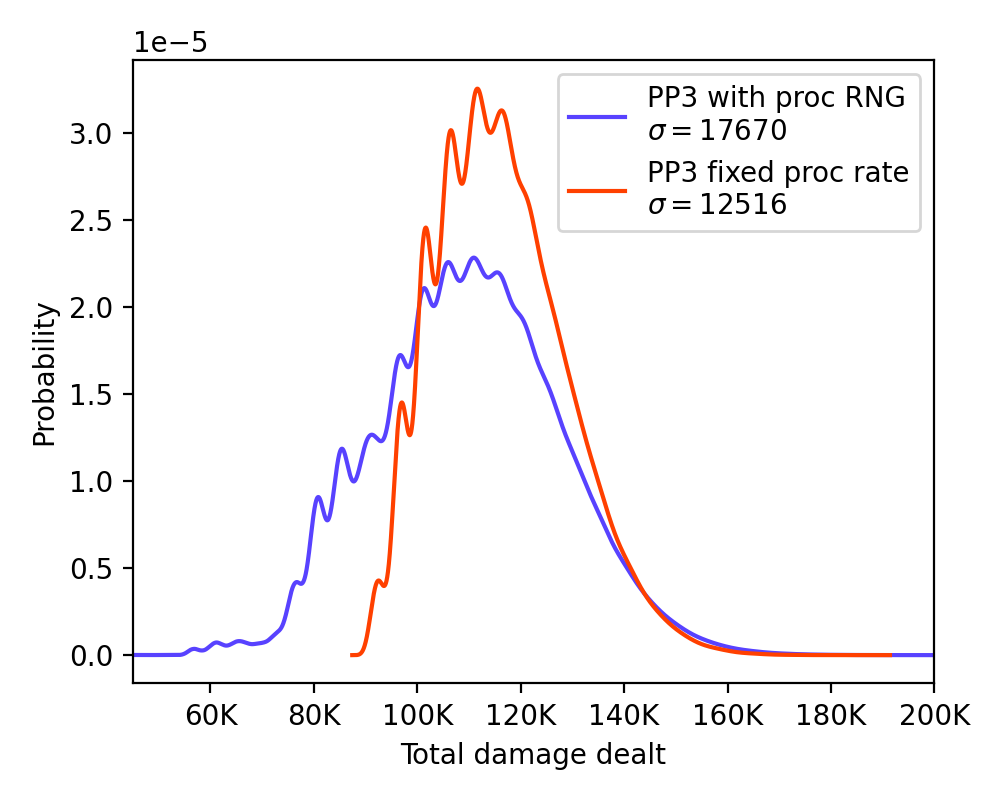
\includegraphics[scale=0.65]{img/wm-dmg-distribution.png}
    \caption{Damage distribution for PP3 accounting for Repertoire proc variability (blue) and the most probable number of PP3 procs (orange).}
    \label{fig:wm-dmg}
\end{figure}

Similar to Mage's Ballad, accounting for Repertoire procs also increases the standard deviation of the damage distribution by about 41\%. Most of the variability is due to the damage distributions of smaller counts of PP3 procs, which are centered around smaller damage values, now entering into the mixture distribution in eqn. \ref{eqn:pp3-damage-distribution}. The total damage dealt is also about twice the amount compared to HS.
